\chapter{Befestigung der Hardware}
\label{chap:hardware-mounting}
Um die Hardware des AudiTim-Systems sicher und stabil zu befestigen, sind verschiedene Montagemöglichkeiten verfügbar. 
Ein Großes Problem bei vorgefertigten halterungen ist jedoch, dass diese oft an die and geschraubt oder anderweitig befestigt werden müssen.
Daher fiel für unser Projekt die wahl auf eine selbst designte Halterung, welche in einem 3D-Drucker hergestellt werden kann.
Dies Garantiert dass keine schäden an der Hardware oder am Raum in welchem die Hardware montiert wird entstehen.

\section{Platzungskonzept}
Aus akustischer Sicht liefern Messungen die zuverlässigsten Ergebnisse, wenn die Sensoren auf Kopfhöhe im Sitzen (~1,2-1,5 m Höhe) angebracht sind und mindestens 1 Meter Abstand zu Wänden und der Schallquelle haben. 
Dieses Vorgehen minimiert frühe Reflexionen, stehende Wellen und lokale Pegelabweichungen - Faktoren, die die Messgenauigkeit maßgeblich beeinträchtigen \cite{oltheten2019micplacement} .
Leider ist diese ideale Positionierung in unserem Fall praktisch nicht umsetzbar. So birgt Montage am Boden, Tischen oder gesonderte "Ständer" erhöhte Gefahr von Beschädigungen, Verschiebungen und Manipulation.
An der Decke jedoch beifinden sich bereits vorhandene Löcher; diese können genutzt werden, um die Sensoren und den Mikrocontroller sicher zu befestigen. 
Auch den einen Meter Abstand zu Wänden und Schallquellen kann so eingehalten werden.
Dieser Kompromiss ermöglicht eine schützende, wartungsarme und vergleichbare Positionierung der Sensoren.
So bleibt der Messaufbau reproduzierbar, sicher und funktional, auch wenn die akustisch ideale Lösung nicht vollständig umsetzbar ist.

\section{Deckenhalterung}
Um die Hardware an der Decke zu befestigen, wurde eine spezielle Halterung entworfen, die eine sichere Montage ermöglicht.
Diese Halterung nutzt die in den Decken vorhandenen "Löcher" für die Montage und wurde als eine Art Pin konzipiert.

\begin{center}
  \begin{minipage}[b]{0.32\textwidth}
    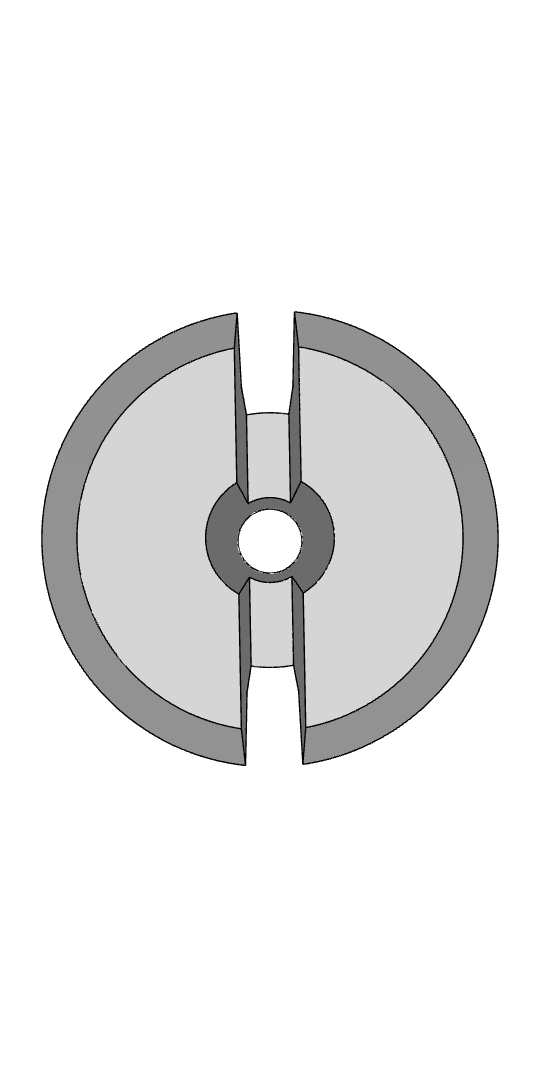
\includegraphics[width=\textwidth]{../images/3DPrinting/Pin1.png}
  \end{minipage}
  \hfill
  \begin{minipage}[b]{0.32\textwidth}
    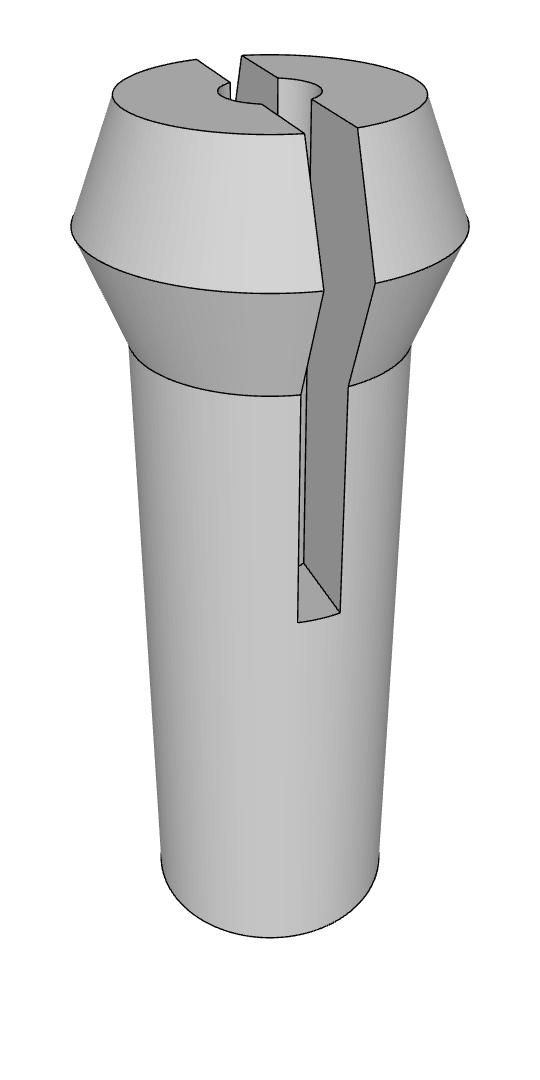
\includegraphics[width=\textwidth]{../images/3DPrinting/Pin2.png}
  \end{minipage}
  \hfill
  \begin{minipage}[b]{0.32\textwidth}
    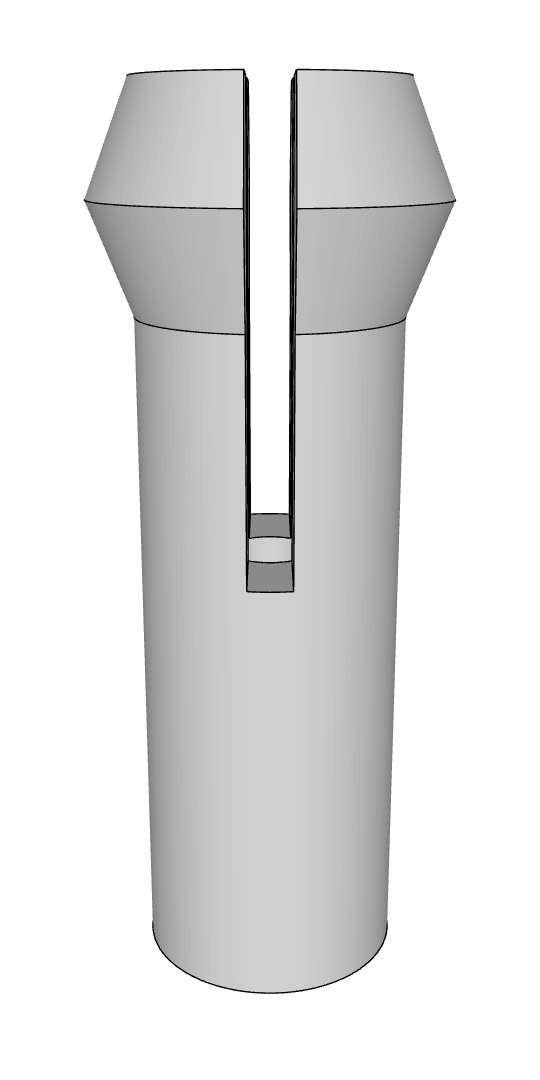
\includegraphics[width=\textwidth]{../images/3DPrinting/Pin3.png}
  \end{minipage}
\end{center}

Der in den Bildern Dargestellte Pin kann durch den Spalt in der Mitte in die öffnung der Decke gesteckt werden.
Durch die Konische form der Spitze des Pins wird garantiert dass dieser auch bei der Demontage des Projekts keine schäden hinterlässt.
Das runde loch welches sich durch den Pin zieht dient dazu, den Pin mit einer Schraube an der Hardware zu befestigen.

\section{ESP32-Halterung}
Der Esp benötigt eine Box welche sicher an der Decke mit den Pins befestigt werden kann.
Bei dem Design der Box wurde sich an einigen Vorlagen orientiert um eine optimale Passform zu gewährleisten.
Die Box ist so gestaltet, dass sie den ESP32 sicher hält und gleichzeitig genug Platz für die Verkabelung bietet.

\begin{center}
  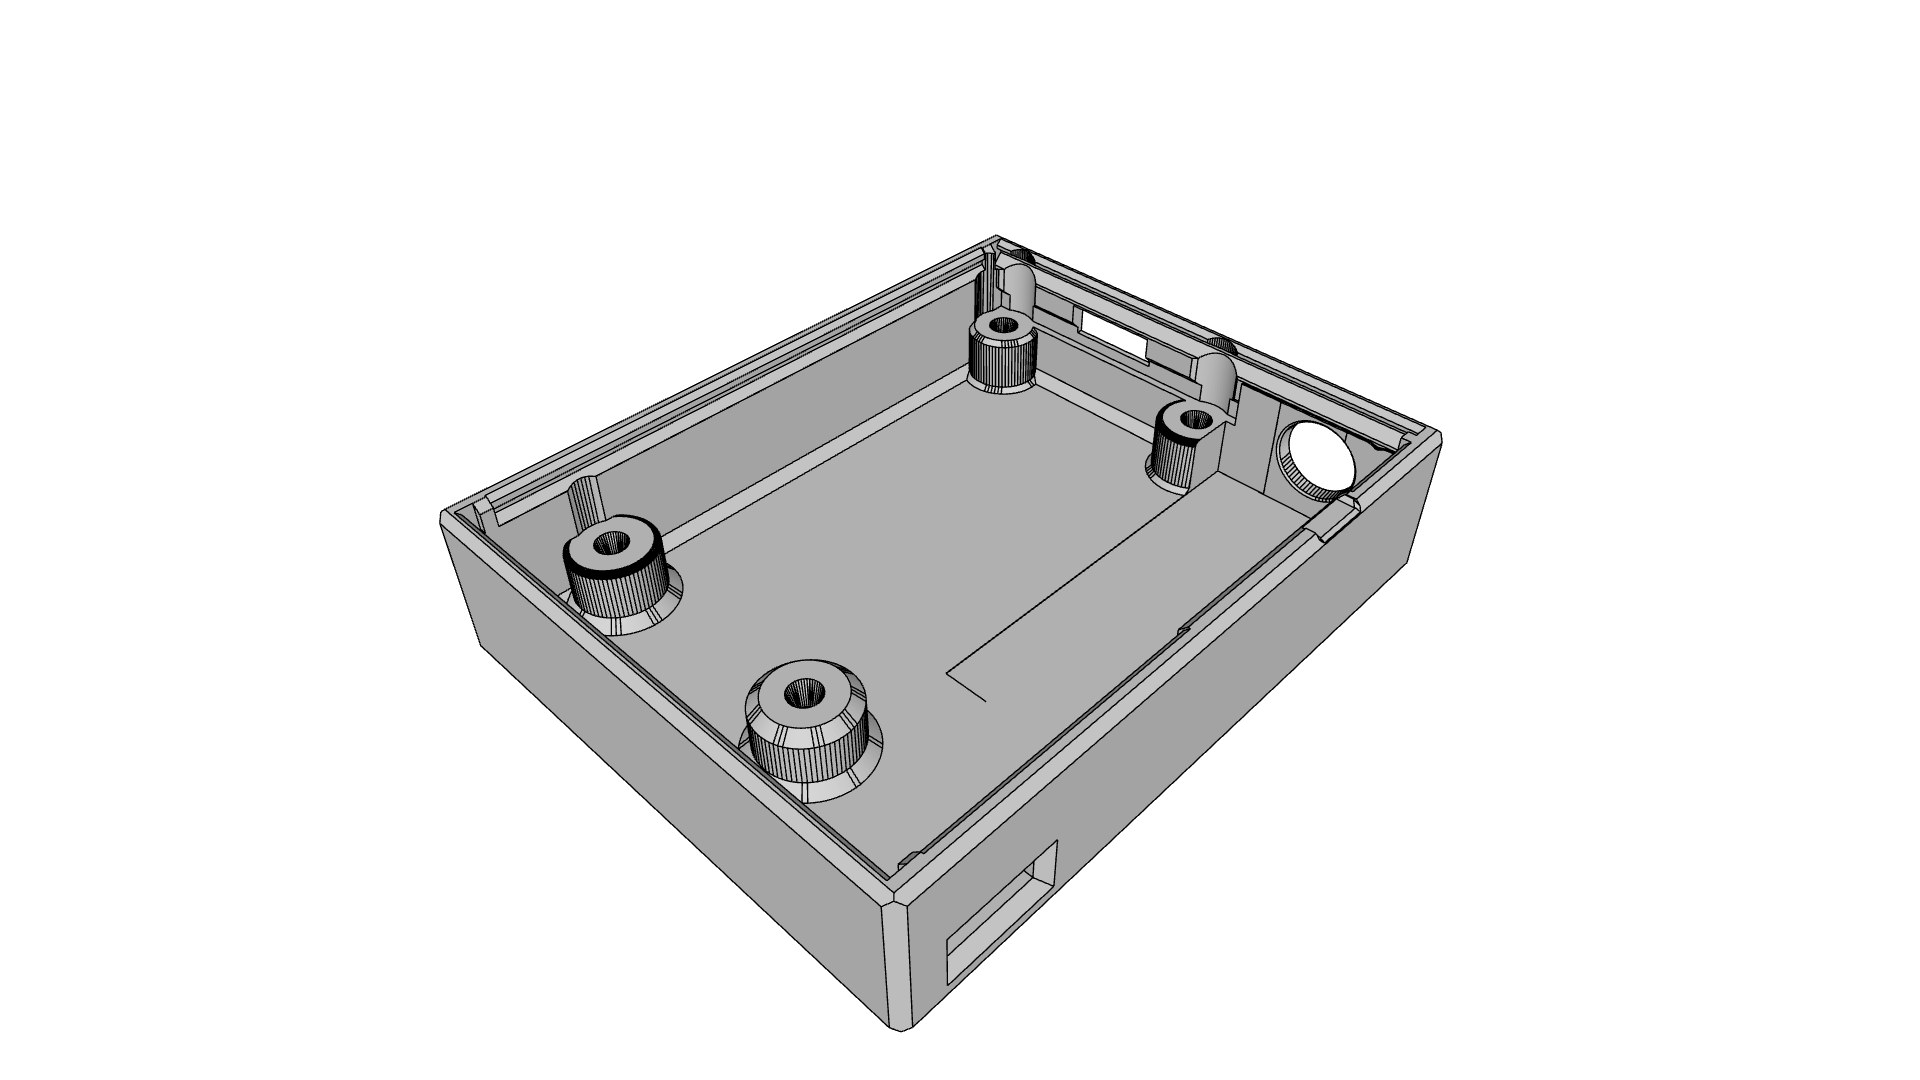
\includegraphics[width=1\textwidth]{../images/3DPrinting/ESPCaseBot.png}
\end{center}

Die angesprochenen löcher der Pins kommen in der Decke der Box zum Einsatz, um die Box sicher an der Decke zu befestigen.
Diese werden durch die löcher in der Decke mit schrauben von innen befestigt.

\begin{center}
  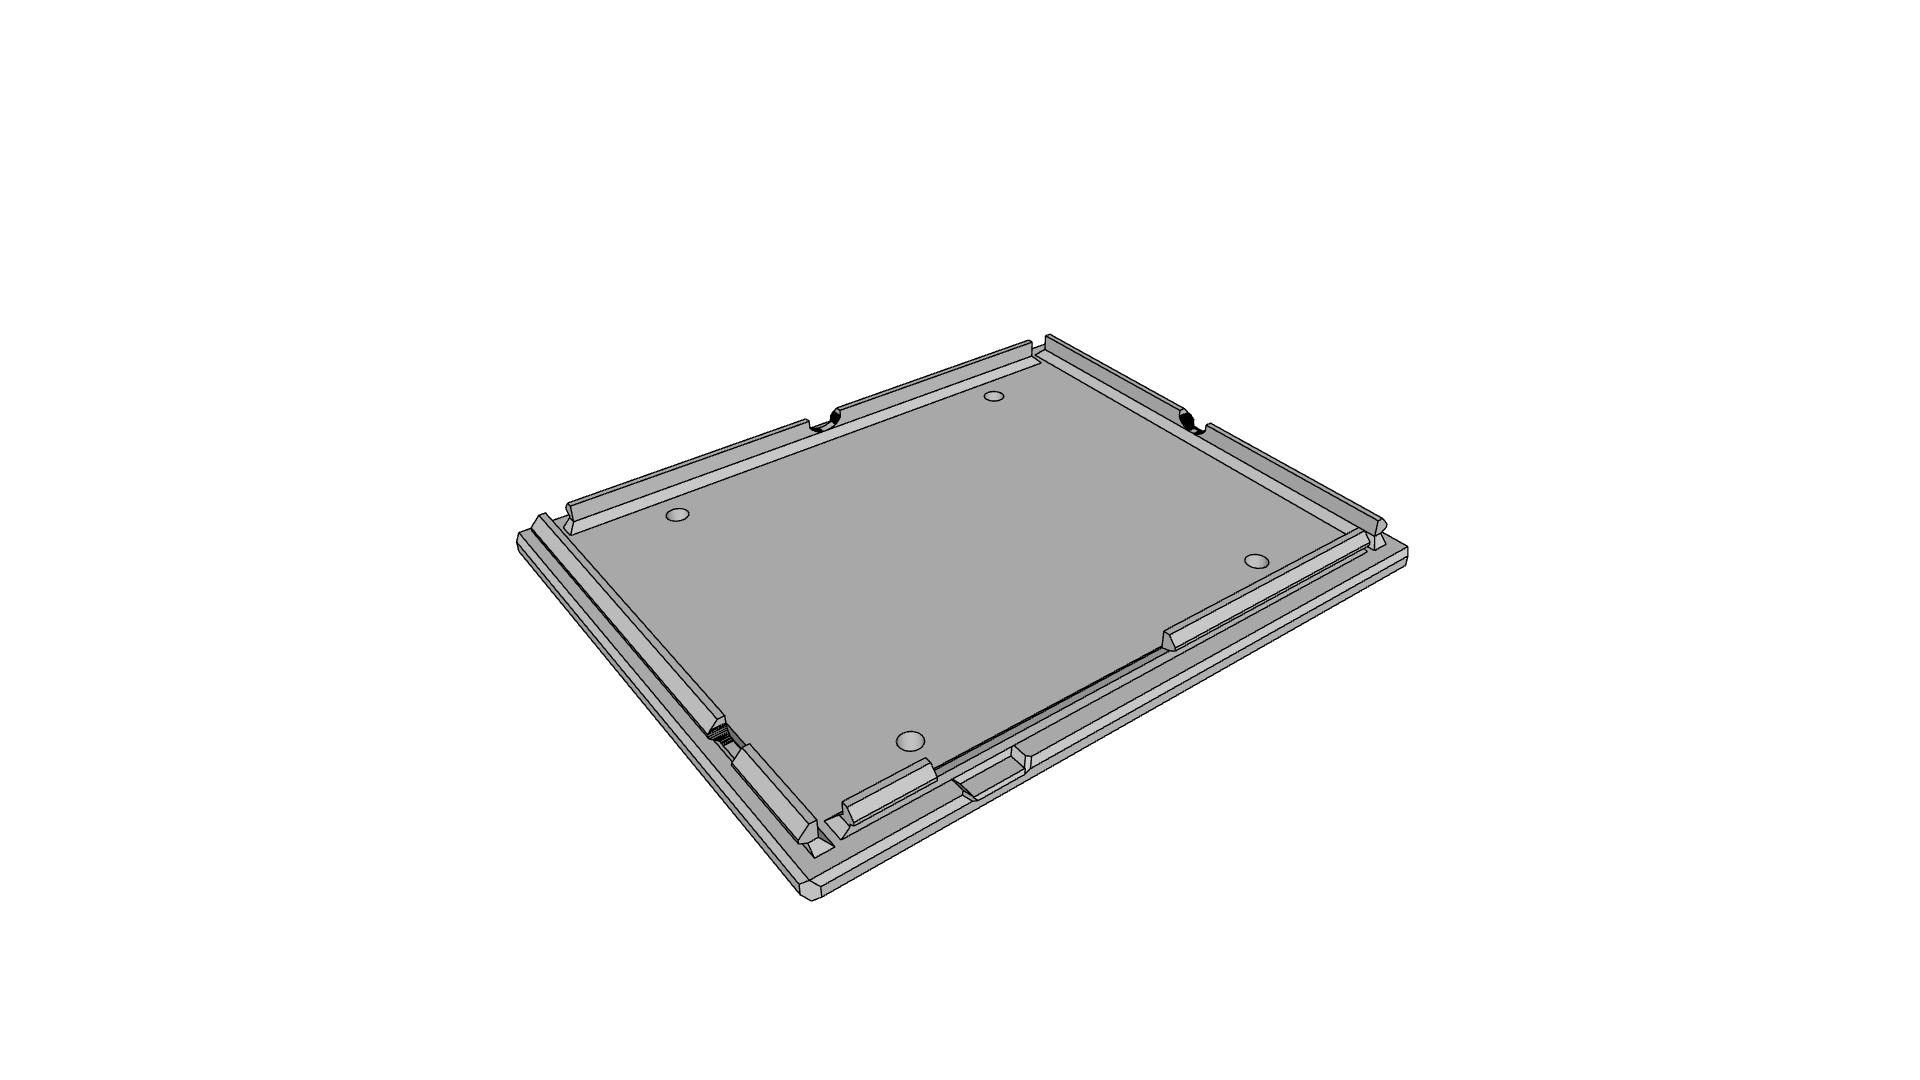
\includegraphics[width=1\textwidth]{../images/3DPrinting/ESPCaseTop.png}
\end{center}

\section{Sensor-Halterung}

Die Sensorhalterung wurde so entworfen dass sie platz für einen möglichen Dämpfer bietet,
welcher um das Mikrofon befestigt werden kann.
Auch diese Halterung wird mit den Pins an der Decke befestigt, jedoch wird sie nicht geschraubt sondern direkt mit den Pins gedruckt.
Der Sensor wird dann einfach mit zwei schrauben an der Halterung befestigt.

\begin{center}
  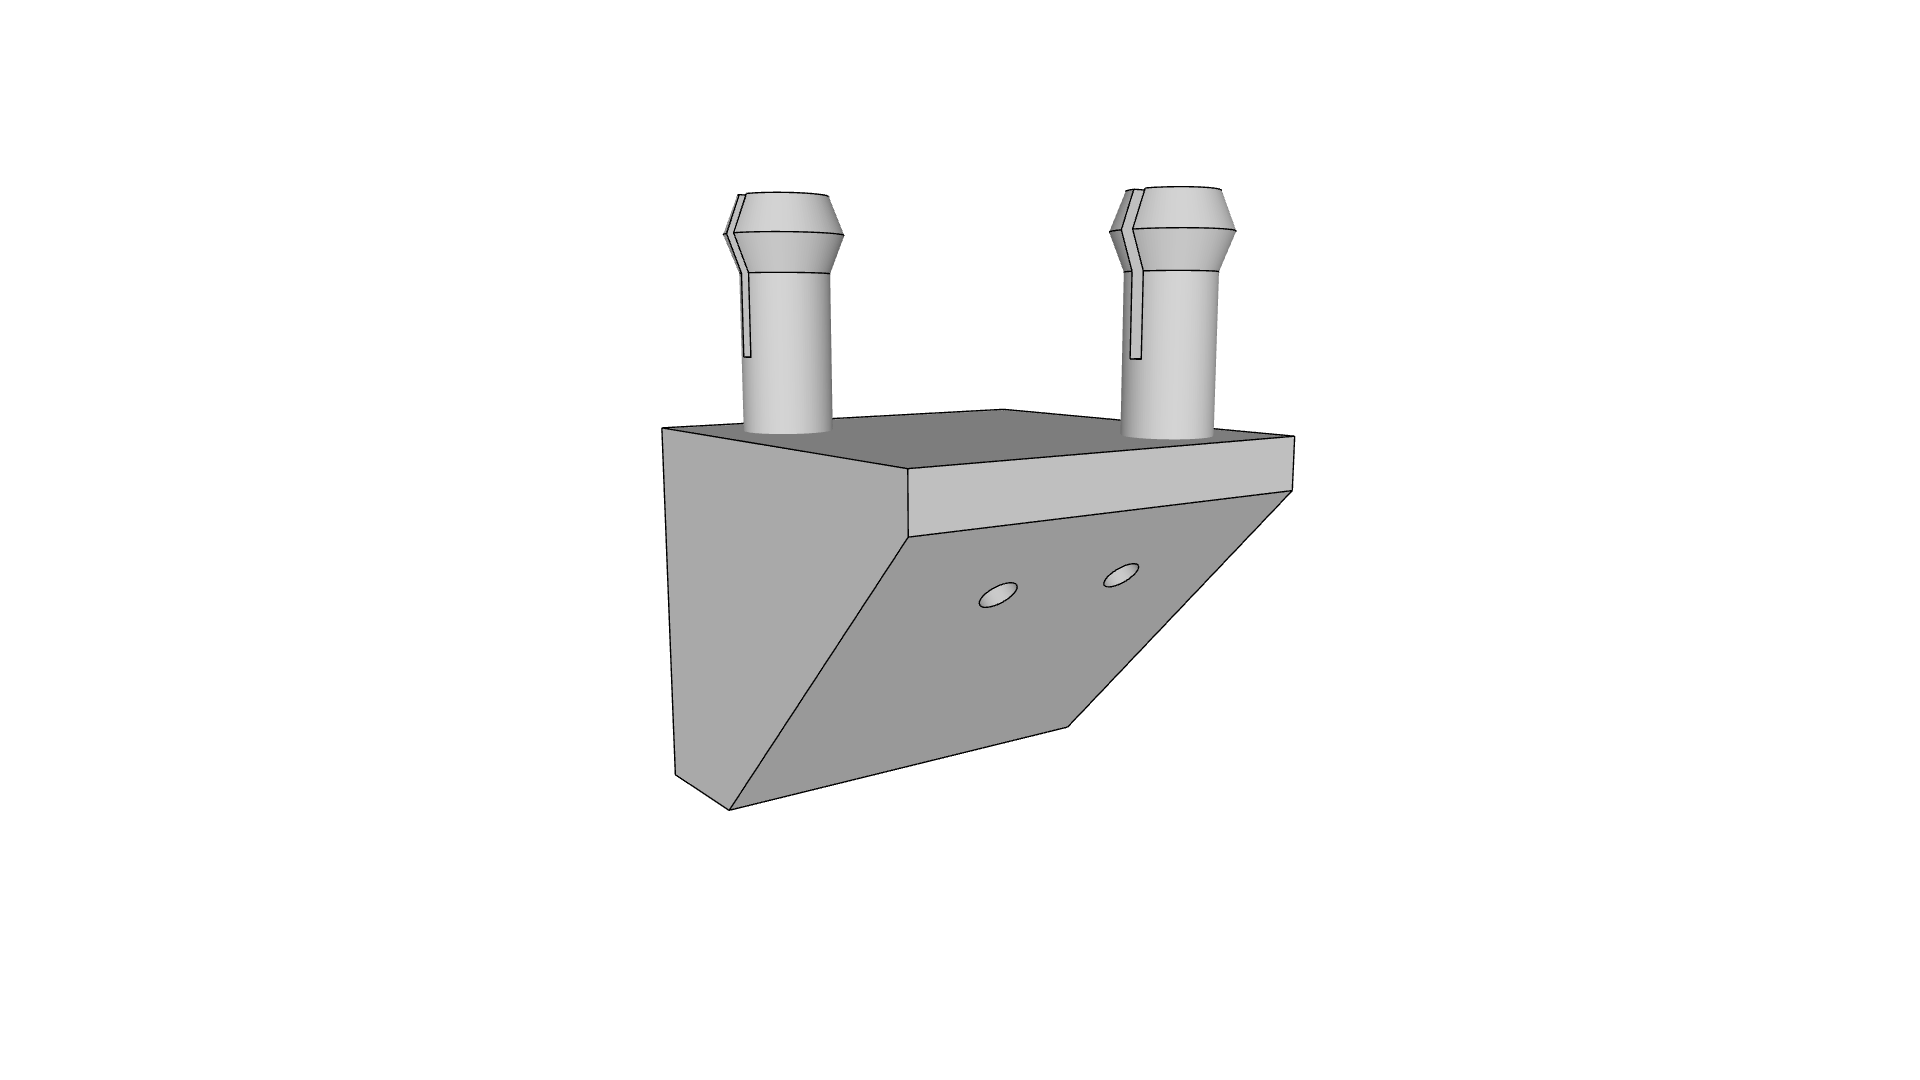
\includegraphics[width=1\textwidth]{../images/3DPrinting/SensorStand.png}
\end{center}

\section{3D-Raummodellierung}
Um eine grafische Übersicht der Montage der ESPs und Sensoren zu erhalten, wurde ein 3D-Modell des Raumes erstellt.
Außderdem soll dieses später als Grundlage für die Simulation der Schallausbreitung als Hintergrund für die Heatmap im Frontend dienen.
Dafür wurde vorerst der Vorlesungsraum ausgemessen und in einer technischen Zeichnung festgehalten:
\begin{center}
  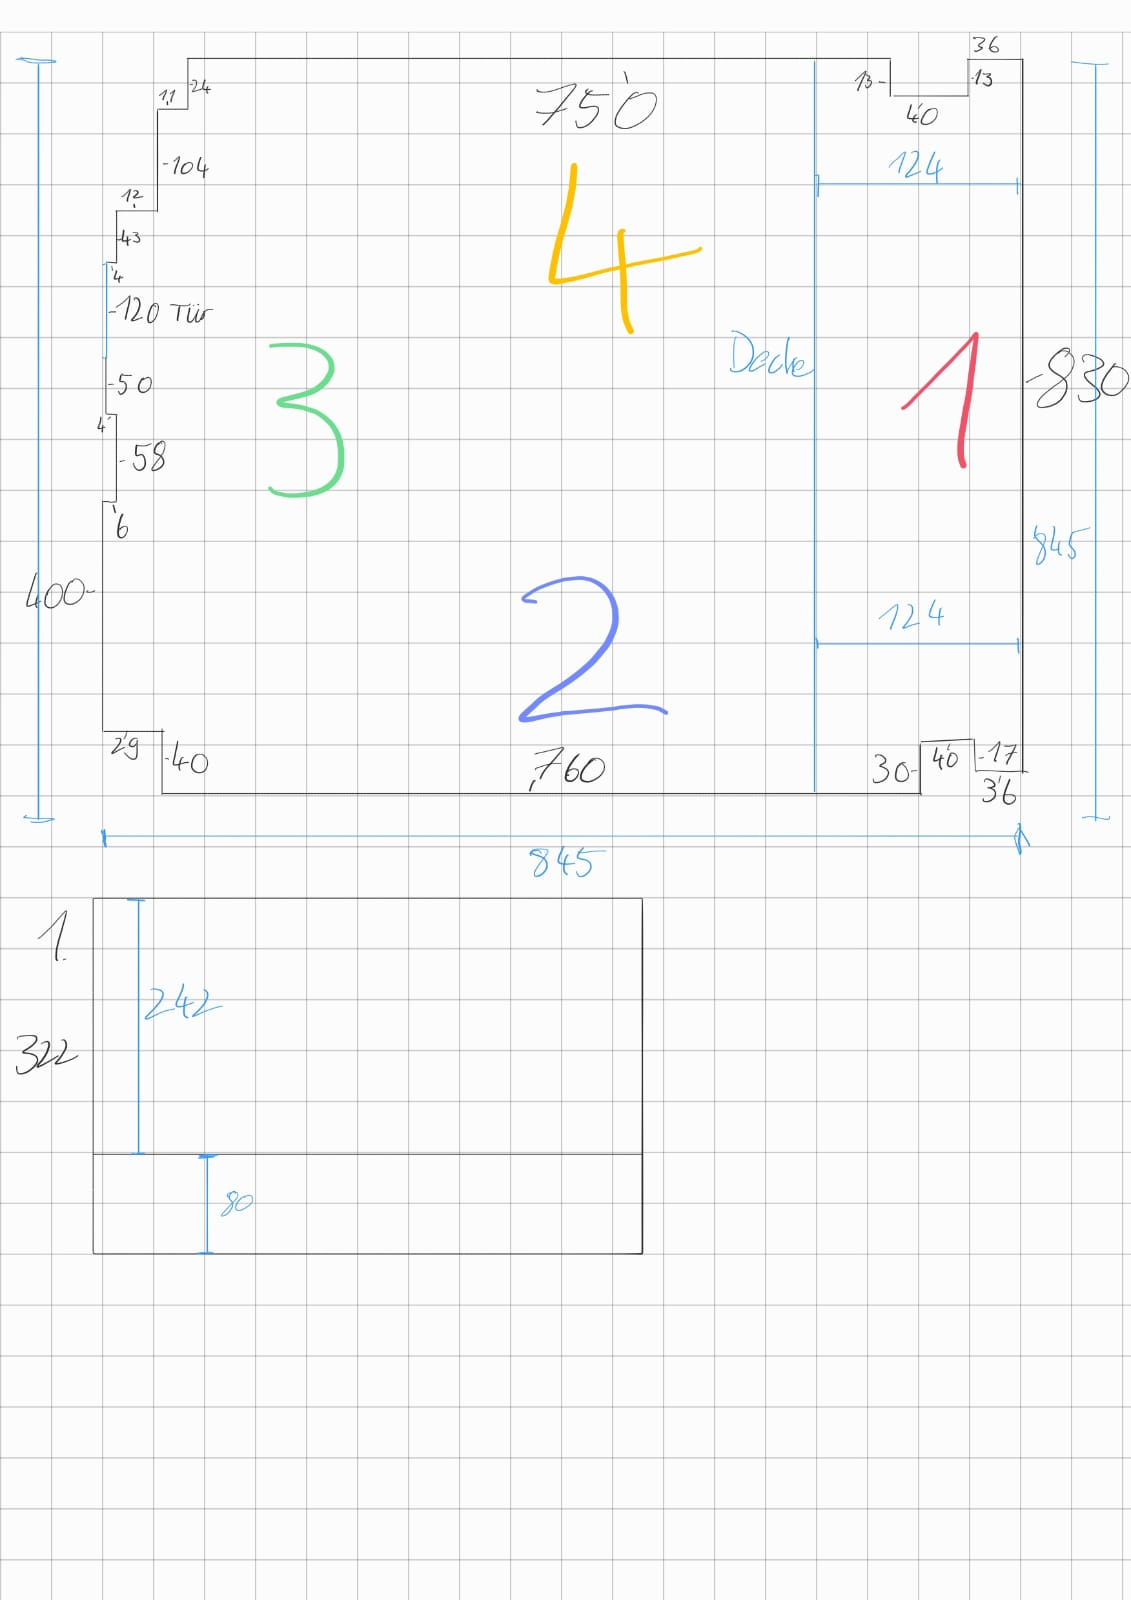
\includegraphics[width=1\textwidth]{../images/3D-Modell/technZeichnVL.jpeg}
\end{center}
Diese Zeichnung dient als Grundlage für die 3D-Modellierung des Raumes, welche in Blender durchgeführt wurde:
\begin{center}
  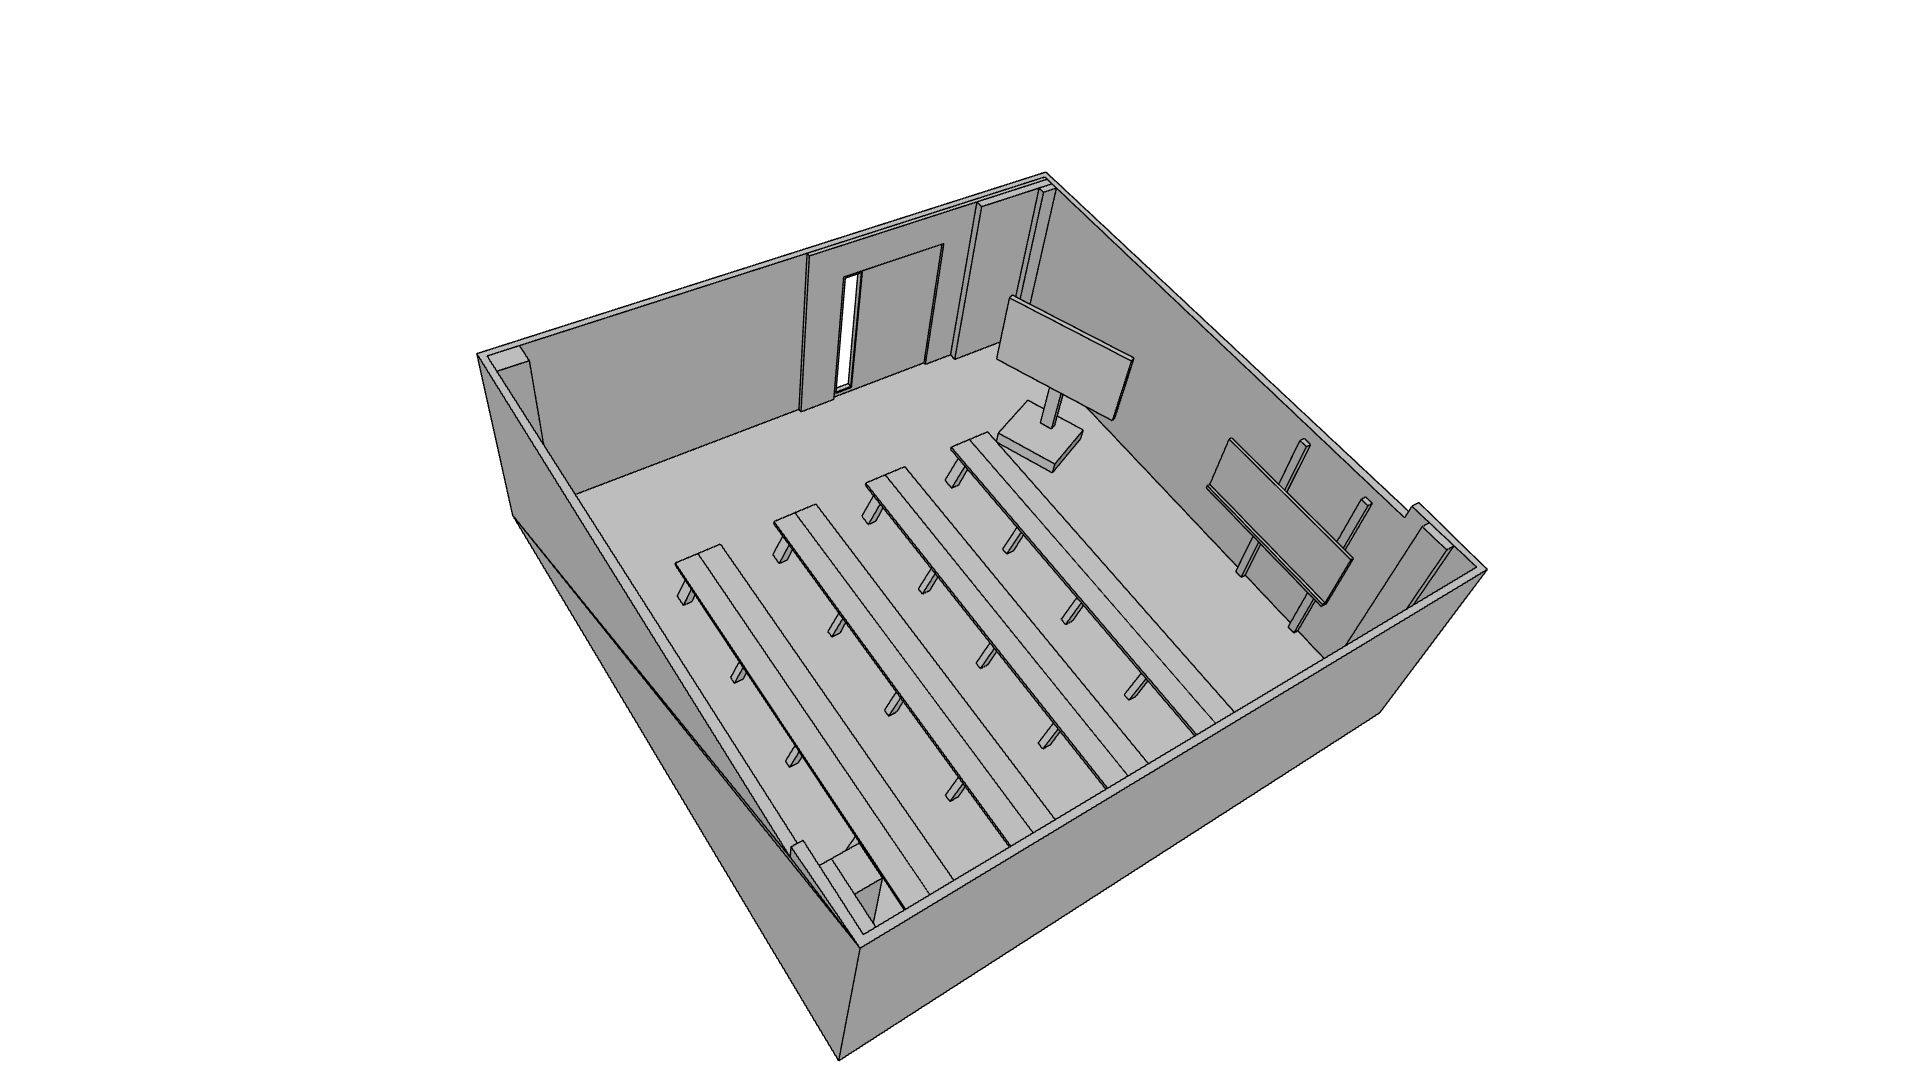
\includegraphics[width=1\textwidth]{../images/3D-Modell/VLModell.png}
\end{center}